%! TEX program = xelatex

\documentclass{article}
\usepackage[a4paper, margin=3cm]{geometry}
\setlength{\parindent}{0pt}
\setlength{\parskip}{1em}
\usepackage{fontspec}
\setmainfont{Lato}

\usepackage{amsmath,amssymb,amsthm}
% \usepackage{hyperref}
\usepackage{graphicx}
% \usepackage{pgfplots}
% \pgfplotsset{compat=1.16}

\usepackage{verbatim}
\usepackage{listings}
\usepackage{xcolor}
\definecolor{purple}{RGB}{135,20,85}
\definecolor{gray}{RGB}{100,100,100}
\lstset{
  basicstyle=\ttfamily,
  keywordstyle=\color{purple},
  commentstyle=\color{gray},
}

\title{TIEA381 Demo 4}
\author{Mikael Myyrä}
\date{\number\day.\number\month.\number\year}

\begin{document}
\maketitle

\section*{1.}

Nyt  $x_0 = 1, x_1 = 2, x_2 = 4, x_3 = 10$
ja $y_i = \log x_i$.
Lasketaan Lagrangen interpolointipolynomin kantafunktiot
\[
  l_j(x) = \prod_{\substack{k=0 \\ k \neq j}}^{n}
    \Big(\frac{x - x_k}{x_j - x_k}\Big)
\]
(Wolfram Alphalla).
\begin{align*}
  l_0(x) &= \frac{(x-2)(x-4)(x-10)}{(1-2)(1-4)(1-10)} = -\frac{1}{27}(x^3 - 16x^2 + 68x - 80) \\
  l_1(x) &= \frac{(x-1)(x-4)(x-10)}{(2-1)(2-4)(2-10)} = \frac{1}{16}(x^3 - 15x^2 + 54x - 40) \\
  l_2(x) &= \frac{(x-1)(x-2)(x-10)}{(4-1)(4-2)(4-10)} = -\frac{1}{36}(x^3 - 13x^2 + 32x - 20) \\
  l_3(x) &= \frac{(x-1)(x-2)(x-4)}{(10-1)(10-2)(10-4)} = \frac{1}{432}(x^3 - 7x^2 + 14x - 8) \\
\end{align*}
Interpolointipolynomi on näiden sisätulo $\mathbf{y}$:n kanssa
\[
  p(x) = \sum_{j=0}^{n} y_jl_j(x).
\]
Tämän likiarvo:
\[
  p(x) \approx 0.010x^3 - 0.187x^2 + 1.220x - 1.005
\]


\section*{2.}

Pisteistö $(1,2),(3,1),(4,3),(6,5),(8,6)$.

Differenssitaulu:
\[
  \begin{array}{c|ccccc}
    x_i & f[x_i] \\
    1 & 2 & \frac{1-2}{3-1} = -\frac{1}{2} & \frac{2+\frac{1}{2}}{4-1} = \frac{5}{6}
      & \frac{-\frac{1}{3}-\frac{5}{6}}{6-1} = -\frac{7}{30}
      & \frac{\frac{1}{24}+\frac{7}{30}}{8-1} = \frac{11}{280} \\
    3 & 1 & \frac{3-1}{4-3} = 2 & \frac{1-2}{6-3} = -\frac{1}{3} 
      & \frac{-\frac{1}{8}+\frac{1}{3}}{8-3} = \frac{1}{24} \\
    4 & 3 & \frac{5-3}{6-4} = 1 & \frac{\frac{1}{2}-1}{8-4} = -\frac{1}{8} \\
    6 & 5 & \frac{6-5}{8-6} = \frac{1}{2} \\
    8 & 6 \\
  \end{array}
\]
Polynomi saadaan ylimmästä rivistä:
\begin{align*}
  p(x) &= 2 - \frac{1}{2}(x-1) + \frac{5}{6}(x-1)(x-3)
    - \frac{7}{30}(x-1)(x-3)(x-4) \\
       & \qquad + \frac{11}{280}(x-1)(x-3)(x-4)(x-6) \\
       &= \frac{11}{280}x^4 - \frac{47}{60}x^3 
       + \frac{1493}{280}x^2 - \frac{793}{60}x + \frac{372}{35} \\
\end{align*}


\section*{3.}

Kolme pistettä $(1,3),(2,4),(5,0)$, joissa toiset derivaatat $M_0$, $M_1$ ja $M_2$.
Luonnolliselle kuutiosplinille $M_0 = M_2 = 0$, jolloin
$M_1$ saadaan yhtälöstä
\[
  \mu_1M_0 + 2M_1 + \lambda_1M_2 = d_1 \iff 2M_1 = d_1 \iff M_1 = \frac{d_1}{2},
\]
missä
\[
  d_1 = \frac{6(\sigma_2 - \sigma_1)}{h_1 + h_2},
\]
\[
  \sigma_i = \frac{y_i - y_{i-1}}{h_i}
\]
ja
\[
  h_i = x_i - x_{i-1}.
\]
Nyt
\begin{align*}
  h_1 &= 2 - 1 = 1, \\
  h_2 &= 5 - 2 = 3, \\
  \sigma_1 &= \frac{4 - 3}{1} = 1, \\
  \sigma_2 &= \frac{0 - 4}{3} = -\frac{4}{3}, \\
  d_1 &= \frac{6(-\frac{4}{3} - 1)}{1 + 3} = -\frac{7}{2}, \\
  M_1 &= \frac{-\frac{7}{2}}{2} = -\frac{7}{4} \\
\end{align*}
Tästä saadaan splinin lausekkeen osat (luentomonisteen kaava 5.20)
\begin{align*}
  s_1(x) &= -\frac{7}{4}\frac{(x-1)^3}{6*1} + 3\frac{2-x}{1}
      + (4-\frac{-\frac{7}{4}*1^2}{6})\frac{x-1}{1} \\
         &= -\frac{7}{24}(x^3 - 3x^2 + 3x - 1) + 6 - 3x + \frac{103}{24}(x-1) \\
         &= -\frac{7}{24}x^3 + \frac{7}{8}x^2 + \frac{5}{12}x + 2 \\
  s_2(x) &= -\frac{7}{4}\frac{(5-x)^3}{6*3}
    + (4-\frac{-\frac{7}{4}*3^2}{6})\frac{5-x}{3} \\
         &= -\frac{7}{72}(-x^3 + 15x^2 - 75x + 125)
          + \frac{159}{24} * \frac{5-x}{3} \\
         &= \frac{7}{72}x^3 - \frac{105}{72}x^2 + \frac{61}{12}x - \frac{10}{9} \\
\end{align*}
Siis koko splini on
\[
  s(x) =
  \begin{cases}
    -\frac{7}{24}x^3 + \frac{7}{8}x^2 + \frac{5}{12}x + 2, \quad 1 \leq x \leq 2 \\
    \frac{7}{72}x^3 - \frac{105}{72}x^2 + \frac{61}{12}x - \frac{10}{9}, \quad 2 \leq x \leq 5
  \end{cases}.
\]

\section*{4.}

Käytetään luentodioista tuttua sisätuloa
\[
  \langle u, v \rangle_{L^2(-1,1)} = \int_{-1}^{1} u(x)v(x)\,dx.
\]
Tarkasteltavan aliavaruuden kanta on $\varphi = (x, x^3, x^5)$,
jolle saadaan kantavektorin indeksistä riippuva kaava
$\varphi_i = x^{2i-1}, i = 1,2,3$.
Nyt Gramin matriisin $\mathbf{A}$ alkiot ovat
\begin{align*}
  a_{ij} &= \langle \varphi_j, \varphi_i \rangle
        = \int_{-1}^{1} x^{2i-1}x^{2j-1}\,dx, \quad i,j=1,2,3 \\
         &= \int_{-1}^{1} x^{2i+2j-2}\,dx \\
         &= \Big[\frac{1}{2i+2j-1}x^{2i+2j-1}\Big]_{x=-1}^{x=1} \\
         &= \frac{2}{2i+2j-1} \\
\end{align*}
Approksimoitava funktio on $f = \arctan(x)$.
Yhtälön oikean puolen vektori on nyt
\begin{align*}
  f_i &= \langle f, \varphi_i \rangle
  = \int_{-1}^{1} \arctan(x)x^{2i-1}\,dx, \quad i=1,2,3. \\
\end{align*}
Lasken nämä Wolfram Alphalla.
Saadaan yhtälöryhmä
\[
  \begin{bmatrix}
    \frac{2}{3} & \frac{2}{5} & \frac{2}{7} \\[0.5em]
    \frac{2}{5} & \frac{2}{7} & \frac{2}{9} \\[0.5em]
    \frac{2}{7} & \frac{2}{9} & \frac{2}{11} \\
  \end{bmatrix}
  \mathbf{c}
  =
  \begin{bmatrix}
    \frac{1}{2}(\pi - 2) \\ \frac{1}{3} \\ \frac{\pi}{6} - \frac{13}{45}
  \end{bmatrix}.
\]
Ratkaisen tämän Octaven interaktiivisella tulkilla.
Saadaan polynomille likiarvo
\[
  p(x) = 0.995983x - 0.292281x^3 + 0.083022x^5.
\]


\section*{5-6.}

$n$-asteinen interpolaatiopolynomi tarvitsee $n+1$ näytepistettä,
joten nyt pisteitä tarvitaan kuusi. Matlab-koodi:

\lstinputlisting[language=Matlab]{w4_5.m}

piirtää (a)-kohdassa

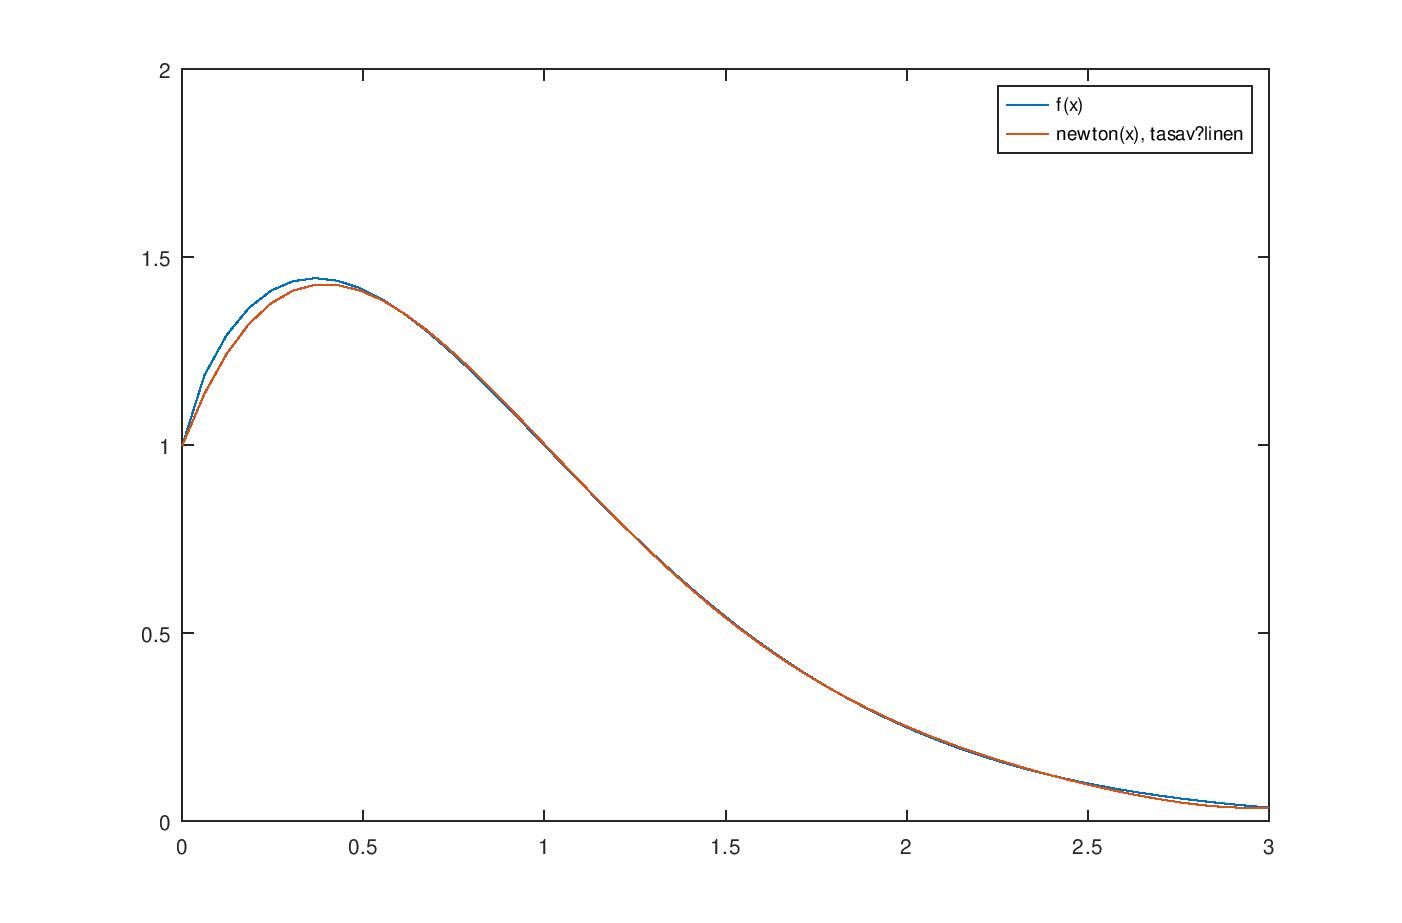
\includegraphics[width=350pt]{w4_5a.jpg}

ja (b)-kohdassa

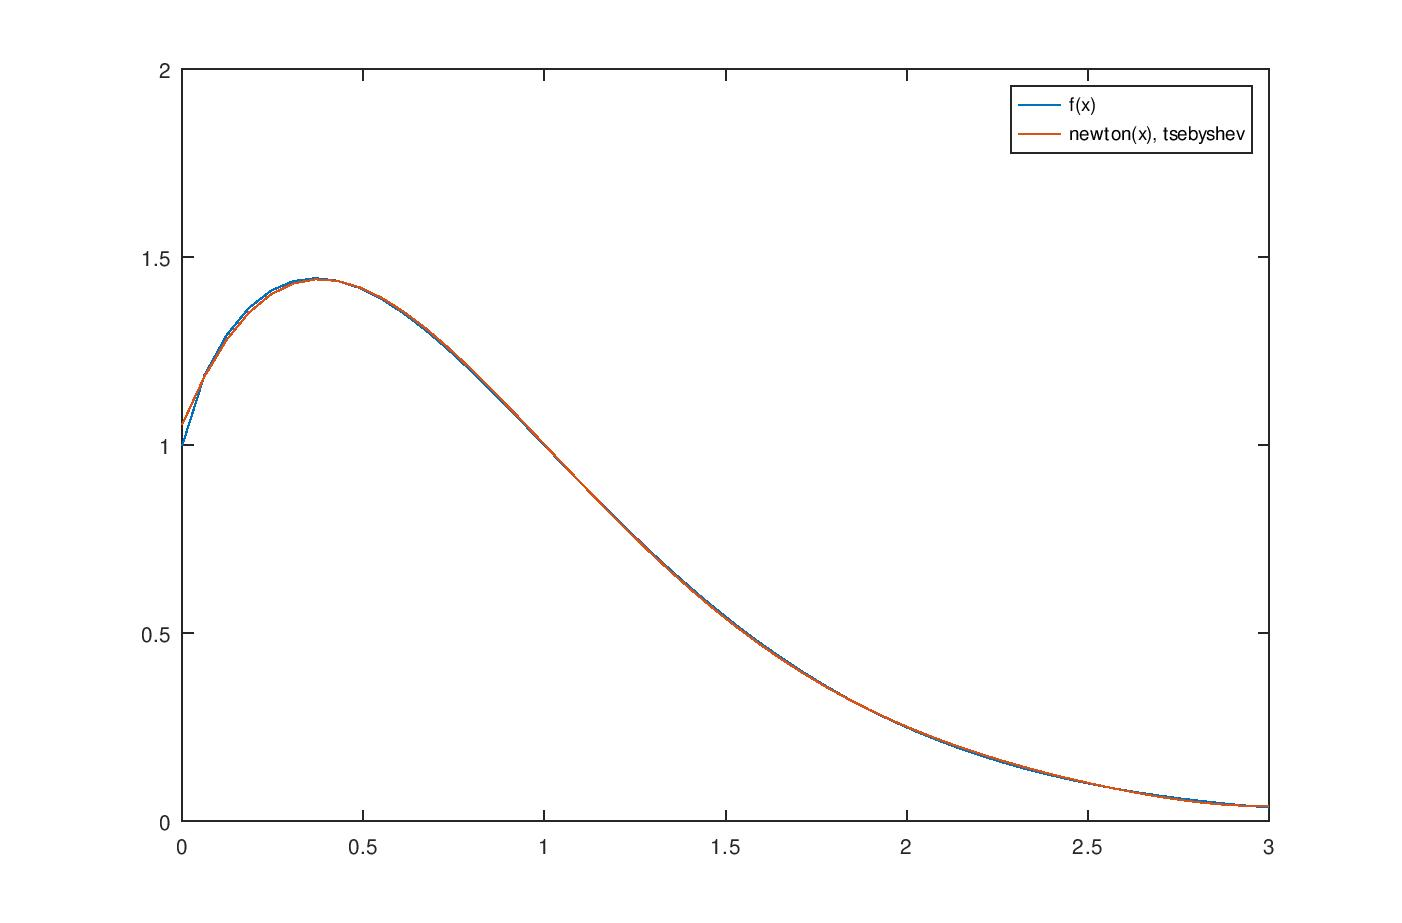
\includegraphics[width=350pt]{w4_5b.jpg}


\end{document}
